
\chapter{Conformación del códec propuesto}\label{capit:cap5}
\vspace{-2.0325ex}%
\noindent
\rule{\textwidth}{0.5pt}
\vspace{-5.5ex}% 
\newcommand{\pushline}{\Indp}% Indent puede ir o no :p

Una vez definidos los conceptos necesarios para el modelado de la parte determinística (Matching Pursuit) y la parte estocástica (Codificación predictiva lineal) del codificador de audio propuesto para este trabajo de tesis, es conveniente mostrar los elementos necesarios para diseñarlo. Para ello, se tomarán los parámetros necesarios de ambos modelados que reconstruyan con precisión la señal de audio cardiaco. 

Una vez obtenidos los parámetros necesarios para conformar el códec es necesario cuantificarlos, este requerimiento es necesario en el sentido de representarlos por medio de palabras código para ser almacenados. La cuantificación es un proceso irreversible de compresión con pérdidas en la codificación de toda señal de audio, el cual por lo tanto debe ser cuidadosamente analizado para que no se distorsionen en gran medida los parámetros que se han cuantificado.

En este capítulo se muestran los pasos necesarios para la conformación del codificador de audio cardiaco; la extracción de los parámetros y su cuantificación. Por último se definirán las tasas de compresión y medidas de distorsión generadas por las señales codificadas para comparar el códec de manera objetiva. 

\section{Estructura del codificador-decodificador propuesto}
Para el desarrollo, modelado y pruebas realizadas al codificador y otros procesos durante este trabajo de tesis se han seleccionado 10 señales de audio cardiaco con duración de 5 segundos desde una base de datos disponible en el sitio web oficial de Litman \copyright, desarrolladores de estetoscopios y otras herramientas de diagnóstico clínico \cite[]{LitmannBase}.

 Se han obtenido las señales indicadas en la Tabla \ref{wavsounds} en formato .wav muestreadas a 11,025 Hz.  Por cuestiones de compatibilidad con los diccionarios en la descomposición las señales han sido remuestreadas a 8,000 Hz.
%--------------------------------------------------------------
\begin{table}[h]
\centering
\begin{tabular}{l}
\hline
\multicolumn{1}{c}{\textbf{Nombre de la señal}}     \\ \hline
División normal del primer ruido (Normal Split S1)  \\ \hline
División normal del segundo ruido (Normal Split S2) \\ \hline
S3                                                  \\ \hline
S4                                                  \\ \hline
Murmullo sistólico temprano (Early Systolic Murmur) \\ \hline
Murmullo sistólico tardío (Late Systolic Murmur)    \\ \hline
Clic de eyección (Ejection Click)                   \\ \hline
Chasquido de apertura (Opening Snap)                \\ \hline
Murmullo pansistólico (Pansystolic Murmur)          \\ \hline
Soplo diastólico (Diastolic Rumble)                 \\ \hline
\end{tabular}
\caption{Sonidos de la base del sitio web Littman \copyright~analizados en este trabajo de tesis. Tomados de \cite[]{LitmannBase}.}
\label{wavsounds}
\end{table}
 %--------------------------------------------------------------
 
El codificador de audio propuesto para este trabajo de tesis consta de los dos modelados matemáticos básicos mostrados en los capítulos anteriores (MP y LPC). 

La Figura \ref{diagEncod} muestra la estructura del codificador diseñado, cuyas etapas serán brevemente explicadas en esta sección. El canal de distribución y/o almacenamiento no será referido durante este trabajo.

Por otra parte, en la Figura \ref{diagDecod} se muestra el procedimiento de decodificación, cuyas etapas son las necesarias para la conformación de la señal de audio reconstruida, la cual será analizada en términos de porcentaje de compresión, distorsión y niveles de error cuadrático medidos desde la señal de audio cardiaco original. 
% ------------------------------------------------
\begin{figure}[h!]
  \centering
  \includegraphics[scale=0.46]{codificador.png}
  \caption{Estructura del codificador para audio cardiaco propuesto.}
  \label{diagEncod}
\end{figure}
% ---------------------------------------------
% ------------------------------------------------
\begin{figure}[h!]
  \centering
  \includegraphics[scale=0.46]{decodificador.png}
  \caption{Estructura del decodificador para audio cardiaco propuesto.}
  \label{diagDecod}
\end{figure}
% ---------------------------------------------
\section{Segmentación de los eventos cardiacos}
El proceso de codificación de audio cardiaco inicia con la \emph{segmentación}, tarea que consiste en extraer los instantes de tiempo (ya sea en segundos o en muestras) donde comienza (\emph{onset}) y termina (\emph{offset}) un sonido o evento cardiaco. La precisión en la localización de estos intervalos es importante\footnote{Esto es, que los valores obtenidos difieran en pocas muestras.}. El diseño del algoritmo automático de segmentación no es parte de los objetivos de este trabajo de tesis, por lo tanto se ha realizado de manera manual.
%-------------------------------------------------
\begin{figure}[ht]
  \centering
  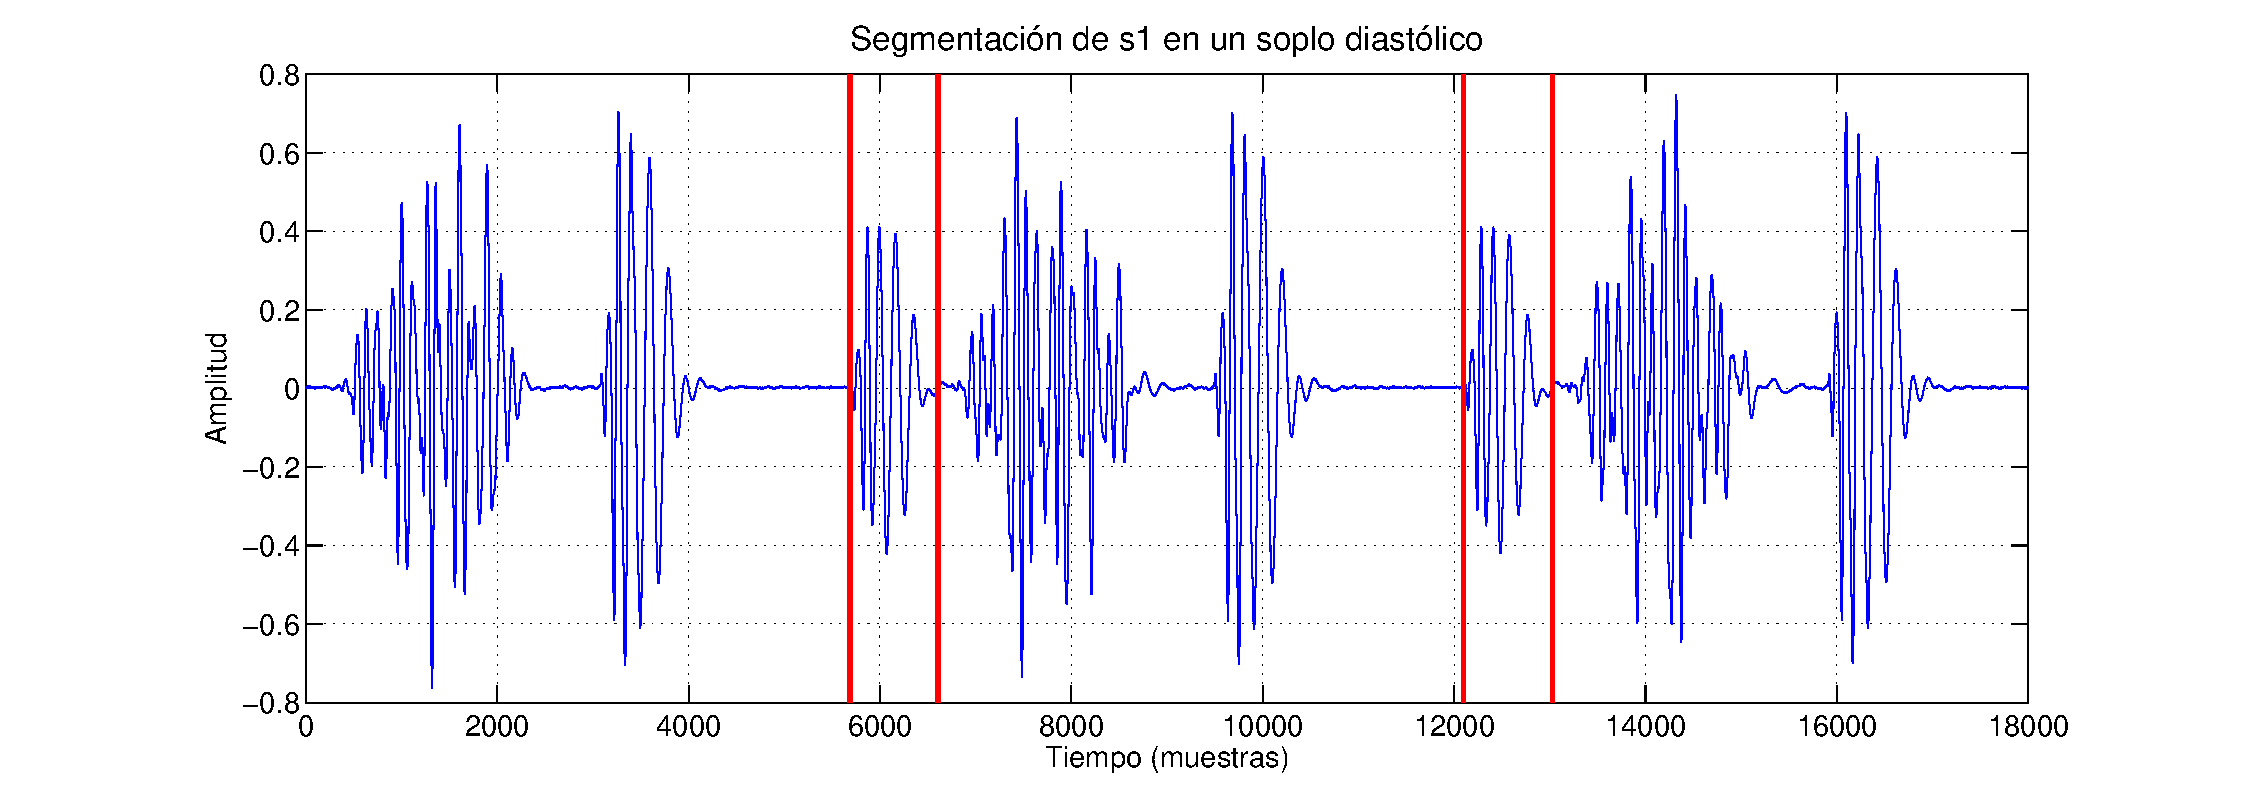
\includegraphics[scale=0.46]{segmentacion.eps}
  \caption{Segmentación del evento cardiaco normal S1 en una señal de audio cardiaco.}
  \label{segment}
\end{figure}
%-------------------------------------------
\section{Descomposición atómica de los eventos (MP)}
Como se ha especificado en el capítulo 3, el proceso de descomposición atómica dado por Matching Pursuit otorga una reconstrucción y compresión aceptables para los eventos cardiacos. La selección de un diccionario \emph{multi-bloques} de Gabor en la descomposición otorga una diversidad atómica en cuanto a frecuencias, posiciones y tamaños de los átomos para la regeneración del evento \cite[]{Nieblas2014}.

\textbf{The Matching Pursuit Toolkit (MPTK)} es una herramienta eficiente en el análisis y síntesis de señales de audio por la técnica Matching Pursuit \cite[]{Krstulovic2006}. La gran ventaja de la herramienta MPTK se basa en la rapidez para calcular las correlaciones (productos internos) entre los átomos del diccionario y las estructuras locales de la señal. Los productos internos son calculados auxiliándose en la FFT y además son actualizados para no re-calcularse (se han preservado en instantes de tiempo anteriores).

En el codificador diseñado para este trabajo de tesis se han realizado las descomposiciones de los eventos cardiacos mediante MPTK y se han seleccionado diccionarios multi-bloques de Gabor como sugiere el trabajo de tesis de \cite{Nieblas2014}. Se trata de dos diccionarios con 4 y 5 bloques respectivamente con las siguientes características que se muestran en la Tabla \ref{dicts}.
% ----------------------------------------------------------------------------------
\begin{table}[h]
\centering
\begin{tabular}{cll}
\hline
\textbf{Parámetros del diccionario}                                                       & \multicolumn{1}{c}{Diccionario 1}                           & \multicolumn{1}{c}{Diccionario 2}                                 \\ \hline
\begin{tabular}[c]{@{}c@{}}Longitudes de las ventanas y \\ átomos (muestras)\end{tabular} & \begin{tabular}[c]{@{}l@{}}64, 128, 256,\\ 512\end{tabular} & \begin{tabular}[c]{@{}l@{}}64, 128, 256,\\ 512, 1024\end{tabular} \\ \hline
\begin{tabular}[c]{@{}c@{}}Tamaños de la FFT\\ (muestras)\end{tabular}                    & \begin{tabular}[c]{@{}l@{}}64, 128, 256,\\ 512\end{tabular} & \begin{tabular}[c]{@{}l@{}}64, 128, 256,\\ 512, 1024\end{tabular} \\ \hline
Tipo de ventana                                                                           & \multicolumn{1}{c}{gaussiana}                               & \multicolumn{1}{c}{gaussiana}                                     \\ \hline
\begin{tabular}[c]{@{}c@{}}Desplazamiento de la\\ ventana (muestras)\end{tabular}         & 8, 16, 24, 32                                               & \begin{tabular}[c]{@{}l@{}}8, 16, 24, 32,\\ 64\end{tabular}       \\ \hline
\end{tabular}
\caption{Características de los diccionarios empleados en la descomposición de los eventos cardiacos del codificador.}
\label{dicts}
\end{table}
% ------------------------------------------------------------------------------

Además, en la Tabla \ref{dicts}, se observa que es conveniente fijar como iguales las longitudes de los átomos y los tamaños de las transformadas rápidas de Fourier (FFT). Esto dará consistencia en las frecuencias atómicas encontradas tras la realización del máximo del producto interno. 

Otro aspecto importante a verificar de los diccionarios es el empalme u \emph{overlap} dado por el corrimiento de la ventana. En este caso las ventanas se irán desplazando por la estructura de la señal en $1/8$ de muestras con relación a su tamaño para calcular las correlaciones correspondientes.

La Figura \ref{MPDecomp} muestra la descomposición mediante MP de un evento cardiaco normal s1 tras realizar 30 iteraciones. Se muestran los primeros 15 átomos seleccionados del análisis ya que presentan mayor amplitud. Se observan en la Figura las diferentes posiciones y frecuencias atómicas (frecuencias de modulación del coseno).
% ------------------------------------------------
\begin{figure}[ht]
  \centering
  \includegraphics[scale=0.38]{MP_decomp.eps}
  \caption{Descomposición MP de un evento cardiaco y muestra de los primeros 15 átomos mayormente correlacionados.}
  \label{MPDecomp}
\end{figure}
% ---------------------------------------------

La Tabla \ref{atoms} muestra el número de eventos y la cantidad de átomos requerida para las descomposiciones Matching Pursuit de las señales de la base de datos. Se observa que la señal del murmullo pansistólico es la que más iteraciones requiere para su representación (392 átomos). Sin duda alguna esta señal presentará menor índice de compresión, dado que la cantidad de átomos es proporcional a la cantidad de bits requeridos para su codificación.

\begin{table}[h]
\centering
\begin{tabular}{lcc}
\hline
\multicolumn{1}{c}{\textbf{Nombre de la señal}} & \textbf{\begin{tabular}[c]{@{}c@{}}Cantidad de \\ eventos\end{tabular}} & \textbf{\begin{tabular}[c]{@{}c@{}}Total de \\ átomos\end{tabular}} \\ \hline
Soplo diastólico                                & 17                                                                      & 264                                                                 \\ \hline
Clic de eyección                                & 19                                                                      & 275                                                                 \\ \hline
Murmullo sistólico temprano                     & 20                                                                      & 365                                                                 \\ \hline
Murmullo sistólico tardío                       & 20                                                                      & 340                                                                 \\ \hline
Chasquido de apertura                           & 19                                                                      & 223                                                                 \\ \hline
S3                                              & 19                                                                      & 197                                                                 \\ \hline
S4                                              & 20                                                                      & 208                                                                 \\ \hline
Murmullo pansistólico                           & 21                                                                      & 392                                                                 \\ \hline
Apertura normal S1                              & 12                                                                      & 130                                                                 \\ \hline
Apertura normal S2                              & 12                                                                      & 172                                                                 \\ \hline
\end{tabular}
	\caption{Cantidad de eventos y número de átomos requeridos en las descomposiciones MP para las señales de la base de datos.}
	\label{atoms}
\end{table}





\section{Modelado y tratamiento de la señal residual (LPC)}

Matching Pursuit, a pesar de ser un algoritmo codicioso (\emph{greedy}) presenta limitantes en cuanto a criterios de selección del número de átomos (iteraciones) o SNR deseada, como se ha mencionado en el capítulo 3. También se ha mencionado que en la práctica el número $N$ de iteraciones nunca es suficiente para representar o retener el 100\% de la energía de la señal analizada, teniendo en la señal residual $R_{M}(t)$ energía aún perceptible para el oído humano dado su comportamiento logarítmico.

En efecto $R_{M}(t)$ presenta correlación muy baja con los átomos de Gabor del diccionario seleccionado, lo cual puede observarse en requerir un gran número de iteraciones sin modelar con éxito esta señal, la cual es considerada por lo tanto como la \emph{parte estocástica} de este codificador de audio.

Es a través de las técnicas de codificación predictiva lineal (LPC) como se ha modelado a la señal residual más silencios del fonocardiograma para el codificador diseñado en esta tesis, parte que se ha establecido que aún contendrá el 1\% de la energía de cada evento del PCG. El criterio de selección de $N$ iteraciones nos da como promedio 10 átomos seleccionados por evento normal y un máximo de 30 átomos por patología o evento de anomalía cardiaca. La Figura \ref{residual} muestra la forma de onda de una señal de soplo diastólico y su señal residual más silencios correspondiente tras realizar el criterio de descomposición antes mencionado.
% ------------------------------------------------
\begin{figure}[ht]
  \centering
  \includegraphics[scale=0.42]{extraccion_residual.eps}
  \caption{Señal de residual y silencios obtenida de un audio cardiaco soplo diastólico.}
  \label{residual}
\end{figure}
% ---------------------------------------------
\subsection{Segmentación del residual}
El análisis LPC de una señal de audio debe realizarse sobre tramos relativamente estacionarios, lo cual reduce la posibilidad de tener cambios abruptos en la autocorrelación y por lo tanto menor cantidad de error en los coeficientes predictores.
Para la señal residual más silencios de audio cardiaco fue necesario tomar tramos de señal de 256 muestras (equivalentes a 32 ms de señal si se considera una frecuencia de muestreo de 8kHz) y posteriormente multiplicarlos por ventanas de análisis tipo \emph{Blackman} para evitar fugas espectrales. 

El empalme u \emph{overlap} de los segmentos analizados fue de 128 muestras (50\%) para asegurar consistencia en la reconstrucción. Se muestra en la Figura \ref{windowing} una descripción gráfica del proceso de segmentación (ventaneo) de la señal residual más silencios cardiacos. 
% ------------------------------------------------
\begin{figure}[ht]
  \centering
  \includegraphics[scale=0.38]{OLA_plot.eps}
  \caption{Ventaneo (segmentación) de la señal residual más silencios.}
  \label{windowing}
\end{figure}
% ---------------------------------------------

 Las tramas de señal obtenidas en el ventaneo son sometidas al análisis LPC, donde será importante extraer los siguientes parámetros para el filtro de síntesis o reconstrucción:
 \begin{itemize}
 	\item Coeficientes predictores $a_{k}$: Calculados mediante la recursión de Levinson por el método de autocorrelación como se mostró en el 			capítulo anterior. El criterio para determinar el número de coeficientes (orden del filtro) se especificará en el siguiente apartado.
	\item Ganancia del filtro predictor: Obtenida para cada trama por la autocorrelación en el instante $t=0$, esto es $\textbf{R}(0)$.
	\item El periodo tonal o pitch: Que se ha obtenido en este trabajo por medio de estimación a través de la función de autocorrelación (ACF) de la 			trama de residual de entrada (máximo de la ACF no ubicado en cero).
 \end{itemize}
 \subsection{Criterios para la determinación del orden $p$ del filtro predictor}
 El filtro predictor lineal es un bloque que se dice \emph{blanquea} o \emph{aplana} el espectro en potencia de la señal de entrada, esto debido a que remueve las correlaciones a corto término.
 La calidad de un filtro predictor se basará en calcular qué tanto es capaz de \emph{aplanar} un espectro en potencia, con lo cual, determinará el grado de tonalidad de un sonido o bien cuánto éste tiende a parecerse a ruido blanco (el cual tiene un espectro plano). Esta medida puede ser obtenida por medio de la \textbf{planitud} o \textbf{aplanamiento espectral}, conocida como \emph{spectral flatness measure} en Inglés. Se denotará en este caso por sus siglas SFM \cite[]{Jayant1974}.
 
 La SFM, $\gamma_{x}^{2}$ se calcula como la razón entre la media geométrica y la media aritmética de la densidad espectral de energía $S_xx(e^{j\omega})$ de una señal de audio:
 %--------------------
 \begin{equation}
 	\gamma_{x}^2 = \frac{\exp\left[\frac{1}{2\pi} \int_{-\pi}^{\pi}\log_{e}S_{xx}(e^{j\omega})d\omega]\right]}{\frac{1}{2\pi}\int_{-\pi}^{\pi}S_{xx}(e^{j\omega})d\omega}.
 \end{equation}
 %--------------------- 
Para la determinación del orden del filtro predictor en la señal residual de audio cardiaco se calculó la SFM promedio de la señal error de cada trama (esta es la salida del predictor lineal) para órdenes predictores $p=1,2,...,100$. Las tramas de audio fueron separadas de acuerdo a si contenían evento cardíaco o presentaban sólo silencio.

De acuerdo a la Figura \ref{sfm}, se ha considerado un aplanamiento aceptable (próximo a volverse constante) a partir de un orden $p=15$ en tramas de silencio cardiaco y tramas con evento respectivamente. 
% ------------------------------------------------
\begin{figure}[ht]
  \centering
  \includegraphics[scale=0.41]{sfm.eps}
  \caption{Medida de planitud espectral promedio de la señal error $e(n)$ para órdenes del filtro predictor desde 1 hasta 100.}
  \label{sfm}
\end{figure}
% ---------------------------------------------
 \subsection{Síntesis/reconstrucción de la señal residual}
 El filtro inverso de reconstrucción IIR por medio de los coeficientes de predicción y la ganancia del filtro predictor reconstruye cada uno de los tramos de señal. Tal como se indicó en el capítulo 4, se presentarán los casos de tener una trama de audio \emph{vocalizada} o \emph{no vocalizada}, excitando al filtro reconstructor con un tren de pulsos separados por el periodo tonal (pitch) en el primer caso y en el segundo mediante ruido blanco gaussiano. 
 
 Una vez regenerados todos los tramos de señal se procede a sintetizar toda la señal de audio cardiaco (contraparte del ventaneo), sumando las partes de los segmentos donde existió el traslape en el ventaneo como se indica en la Figura \ref{OLArecons}. Dicho procedimiento es conocido como \emph{overlap and add (OLA)} en Inglés. 
 % ------------------------------------------------
\begin{figure}[ht]
  \centering
  \includegraphics[scale=0.86]{OLA_recons.pdf}
  \caption{Representación gráfica del procedimiento de síntesis ``overlap and add (OLA)''.}
  \label{OLArecons}
\end{figure}
% ---------------------------------------------
 \subsection{Filtros de pre-énfasis y de-énfasis en LPC}
 La señal de audio cardiaco es pasa-bajas, lo cual indica que en su espectro en potencia a medida que incrementa el rango frecuencial decrece la energía presentada. 
 
 Previo al análisis LPC es conveniente realizar un filtrado de pre-énfasis, cuyo objetivo será realzar las altas frecuencias de la señal y representarlas con una mayor precisión. En la reconstrucción de los segmentos deberá ejecutarse la contraparte de este proceso, el de-énfasis correspondiente que habrá de contrarrestar el efecto. 
 
 Los filtros de pre-énfasis y de-énfasis empleados comúnmente en LPC para los codificadores de voz existentes tienen la siguiente estructura:
 \begin{align}\label{preemph}
 	y(n) = x(n)-a\cdot x(n-1)\\
	y(n) = x(n)+a\cdot x(n-1),
 \end{align}
 donde generalmente se emplea $a=0.9$ en los métodos de predicción lineal.
 
 En la Figura \ref{preem} se muestra la gráfica de la respuesta en frecuencia de los filtros mostrados en \eqref{preemph} y (43), mostrando la parte pasa-altas (pre-énfasis) y pasa-bajas (de-énfasis).
 % ------------------------------------------------
\begin{figure}[ht]
  \centering
  \includegraphics[scale=0.43]{preemp.eps}
  \caption{Filtros de pre-énfasis y de-énfasis usados en la codificación LPC.}
  \label{preem}
\end{figure}
% ---------------------------------------------
\section{Cuantificación}
\subsection{Tipos de cuantificadores}
En la digitalización de una señal de audio está presente un proceso irreversible de compresión con pérdidas como la cuantificación, el cual tiene como objetivo \emph{nivelizar} los parámetros obtenidos para su representación binaria. De manera matemática la cuantificación equivale a sumarle ruido y distorsionar consecuentemente la señal de entrada.

El cuantificador más sencillo de diseñar corresponde a aquella fuente de datos cuya distribución de probabilidad (pdf) es uniforme, sin embargo en la realidad esto no siempre ocurre y es conveniente adaptarlo a una función de distribución de probabilidad no uniforme. 

La Tabla \ref{cuantificadores} define los tipos de cuantificadores con respecto a la dimensión de la fuente de datos de entrada así como a su pdf.
% ---------------------------------------------------------------------------------------------
\begin{table}[h]
\begin{tabular}{|l|l|l|}
\hline
\begin{tabular}[c]{@{}l@{}}Parámetro de la \\ fuente de datos\end{tabular}                             & \begin{tabular}[c]{@{}l@{}}Tipo de \\ cuantificador\end{tabular}     & Características                                                                                                                                \\ \hline
\multirow{2}{*}{\begin{tabular}[c]{@{}l@{}}Función de \\ distribución \\ de probabilidad\end{tabular}} & \begin{tabular}[c]{@{}l@{}}Cuantificador \\ uniforme\end{tabular}    & \begin{tabular}[c]{@{}l@{}}Niveles equidistantes.\\ Implementación sencilla.\end{tabular}                                                      \\ \cline{2-3} 
                                                                                                       & \begin{tabular}[c]{@{}l@{}}Cuantificador no \\ uniforme\end{tabular} & \begin{tabular}[c]{@{}l@{}}Niveles variantes en longitud.\\ Menor distorsión introducida.\end{tabular}                                         \\ \hline
\multirow{2}{*}{Dimensión}                                                                             & Cuantificador escalar                                                & \begin{tabular}[c]{@{}l@{}}Vector unidimensional \\ como fuente de entrada.\end{tabular}                                                       \\ \cline{2-3} 
                                                                                                       & Cuantificador vectorial                                              & \begin{tabular}[c]{@{}l@{}}Cuantificación en bloques \\ (vectores de bits) al agrupar \\ diversas fuentes en \\ una sola entidad.\end{tabular} \\ \hline
\end{tabular}
\caption{Tipos de cuantificadores de acuerdo a las características de la fuente de datos de entrada.}
\label{cuantificadores}
\end{table}


% ---------------------------------------------------------------
\subsection{Diseño de un cuantificador no uniforme}
El cuantificador que introducirá la menor distorsión será aquel que sea diseñado proporcionalmente a la función de distribución de probabilidad de la fuente de entrada. 

El error cuadrado promedio de cuantificación $\sigma_{q}^2$ (MSQE) debe ser el mínimo para presentar la menor distorsión posible tras cuantificar y se define como:
\begin{align}\label{msqe}
	\sigma_{q}^2 = \int_{-\infty}^{\infty} (x-Q(x))^2 f_{X}(x)dx
			 = \sum_{i=1}^{M} \int_{b_{i}-1}^{b_{i}} (x-y_{i})^2 f_{X}(x)dx,
\end{align}
donde $x$ es la fuente de entrada, $Q(x)$ la operación de cuantificación, $f_{X}(x)$ la función de distribución de probabilidad de la fuente, $\{ b_{i}\}_{i=1}^M$ las regiones de decisión y $\{ y_{i}\}_{i=1}^M$ los niveles de reconstrucción (mostrados gráficamente en la Figura \ref{quantz}).
 % ------------------------------------------------
\begin{figure}[ht]
  \centering
  \includegraphics[scale=0.43]{cuantificador.pdf}
  \caption{Regiones de decisión y niveles de reconstrucción de un cuantificador.}
  \label{quantz}
\end{figure}
% ---------------------------------------------
\subsubsection{Algoritmo de Lloyd}
Según lo discutido anteriormente el mejor cuantificador no uniforme surge al tener un modelo probabilístico para la fuente, encontrando los valores $b_{i}$ y $y_{i}$ que minimicen lo definido en la ecuación \eqref{msqe}. La derivación parcial de esta ecuación es un camino para lograr esta minimización, con la cual al resolver para $y_{j}$ se tiene:
%---------------
\begin{equation}\label{nivRec}
	y_{j}=\frac{\int_{b_{j}-1}^{b_{j}} xf_{X}(x)dx}{\int_{b_{j}-1}^{b_{j}} f_{X}(x)dx}.
\end{equation}
%-------------
Teniendo que $\int_{-\infty}^{\infty} xf_{X}(x)dx$ es el valor esperado de la fuente de datos $x$, se define que cada punto a la salida $y_{j}$ para cada intervalo de cuantificación es el centroide de la función de probabilidad en ese intervalo. 

Si se realiza el mismo procedimiento en \eqref{msqe}, ahora para $b_{j}$ (igualando a cero la derivada parcial con respecto a este término) se tiene:
%---------------
\begin{equation}\label{regDec}
	b_{j} = \frac{y_{j+1}+y_{j}}{2}.
\end{equation}
%-------------
Con esto se observa que la región de decisión es simplemente el punto medio de dos niveles de reconstrucción vecinos. Al resolver las ecuaciones \eqref{nivRec} y \eqref{regDec} se obtendrán los valores que minimicen el MSQE definido en \eqref{msqe}, desafortunadamente para resolver $y_{j}$ se requieren los valores $b_{j}$ y $b_{j-1}$ y viceversa. 

El algoritmo de Lloyd, desarrollado por Stuart P. Lloyd describe cómo resolver las ecuaciones \eqref{nivRec} y \eqref{regDec} de manera iterativa, obteniendo los valores $b_{j}$ y $y_{j}$ a base de simetría y suponiendo los valores para la primer región de decisión $b_{0}$ como cero, así como suponiendo que la última región $b_{\frac{M}{2}}$ es el valor más grande que puede tener la entrada. 

\subsection{Cuantificación de los parámetros extraídos de los modelados}

Para el desarrollo del códec de audio propuesto se han cuantificado aquellos parámetros que estén en formato de punto flotante para convertirse en enteros con signo. Esto garantizará la correcta representación de los mismos con el menor número de bits posibles. Es necesario determinar ahora de los parámetros extraídos del PCG de los modelados MP y LPC, cuáles es necesario cuantificar y cuáles será necesario codificar directamente (ya que son enteros con signo).
 % ------------------------------------------------
\begin{figure}[ht]
  \centering
  \includegraphics[scale=0.48]{params_cuant.png}
  \caption{Parámetros extraídos de los modelados MP y LPC para el códec. Se indican los parámetros necesarios de cuantificar.}
  \label{params}
\end{figure}
% ---------------------------------------------

De acuerdo a lo observado en la Figura \ref{params}, habrá que diseñar 4 cuantificadores para el códec, correspondientes a las amplitudes y fases de los átomos seleccionados en MP, los coeficientes de líneas espectrales diferenciales (LSFD, obtenidos a través de los coeficientes predictores) y las ganancias de los filtros de predicción de LPC. El primer paso corresponderá a observar las funciones de distribución de probabilidad (pdf) de las variables para posteriormente determinar sus cuantificadores optimizados mediante el algoritmo de Lloyd.

Se han realizado los histogramas normalizados para determinar las funciones de probabilidad de las amplitudes y fases atómicas extraídas desde MPTK para las señales de la base de datos.
 % ------------------------------------------------
\begin{figure}[ht]
  \centering
  \includegraphics[scale=0.42]{histograma_amplitudesFases.eps}
  \caption{Histogramas normalizados (pdf) para las amplitudes y fases de los átomos extraídos en las descomposiciones.}
  \label{histAmpPh}
\end{figure}
% ---------------------------------------------

 % ------------------------------------------------
\begin{figure}[h!]
  \centering
  \includegraphics[scale=0.42]{histograma_LSFDGanancia.eps}
  \caption{Histogramas normalizados (pdf) para los coeficientes LSFD y ganancias del filtro predictor.}
  \label{histLSFD}
\end{figure}
% ---------------------------------------------

En la Figura \ref{histAmpPh} se observa que la distribución de probabilidad de las fases de los átomos es de manera uniforme en el intervalo $[-\pi,\pi]$, siendo necesario diseñar un cuantificador sencillo para esta variable. En el caso de la amplitud se procederá a diseñar con el algoritmo de Lloyd un cuantificador no uniforme basado en su pdf.

Se observa un comportamiento no uniforme en las funciones de probabilidad obtenidas a través de los histogramas de los coeficientes LSFD y ganancia del filtro predictor, esto según la Figura \ref{histLSFD}. De igual manera que con la amplitud, mediante el método de Lloyd se realizará el diseño de estos cuantificadores no uniformes optimizados.

\subsection{Cuantificación de los coeficientes de predicción}
Como se ha manejado anteriormente, los coeficientes obtenidos para la predicción lineal son bastante sensibles a la inestabilidad, por lo tanto su cuantificación no es realizable de manera directa para su transmisión, ya que la distorsión introducida afectaría en gran medida en la síntesis de la señal \cite[]{Noah1984}.

Sin embargo, existen otras representaciones equivalentes de los coeficientes predictores LPC empleadas en algunos vocoders diseñados en la literatura, con las cuales puede realizarse la cuantificación presentando la menor distorsión posible:

\begin{itemize} 
	\item \textbf{Coeficientes reflectores o PARCORS}: Se obtienen directamente a partir de la recursión de Levinson a la par de los coeficientes 				predictores.
	\item \textbf{Coeficientes de relación log-área (log-area ratios o LAR)}: Los coeficientes reflectores $k_{i}$ pueden sufrir transformaciones para expandir su región en el plano polar \cite[]{Viswanathan1975}. 
	
	Una de estas transformaciones es calculada como el logaritmo de la razón de la suma y resta del $i$-ésimo coeficiente reflector, en una representación conocida como relación log-área (LAR), esto es: $$LAR_{i}=\log\frac{1+k_{i}}{1-k_{i}}.$$
	\item \textbf{Pares o frecuencias de líneas espectrales (line spectrum pairs/frequencies, LSF)}: \cite{Itakura1975}, encontró que el polinomio del filtro predictor $A(z)$ tiene	una representación equivalente a partir de un par de polinomios:
					$$A(z) = 0.5[P(z)+Q(z)]$$
					$$P(z) = A(z)+z^{-(p+1)}A(z^{-1})$$
					$$Q(z) = A(z)-z^{-(p+1)}A(z^{-1}).$$
			Las raíces de $P(z)$ y $Q(z)$ ocurren en pares conjugados y se les denomina \emph{frecuencias} o \emph{pares} de 						líneas espectrales.			
	\item \textbf{Pares o frecuencias de líneas espectrales diferenciales (LSFD's)}: \cite{Soong1984a} explotaron la correlación entre LSF's sucesivos, para ello cuantificaron las diferencias entre éstos. A tal representación equivalente se le conoce como LSF diferenciales ó LSFD's:
			$$LSFD_{i}=LSF_{i+1}-LSF_{i}.$$
\end{itemize}
Seleccionar la representación LPC adecuada en el diseño del codificador será una medida que intervendrá en la calidad de la reconstrucción de la señal. La distorsión espectral (medida en decibeles) es una medida que indica la cantidad de degradación del espectro en potencia de la señal analizada tras seleccionar alguna representación equivalente de las antes mencionadas y haber cuantificado. 

 Se define como la distorsión espectral $D_{i}$ común entre dos tramas de audio a la siguiente expresión:
 \begin{equation}\label{spectralDisort}
 	D_{i} = \sqrt{ \frac{1}{f_{s}} \int_{0}^{f_{s}} [10\log_{10}(P_{i}(f))-10\log_{10}(\widehat{P}_{i}(f))]^{2} df  },
 \end{equation}
 donde $f_{s}$ es la frecuencia de muestreo en Hz,  $P_{i}(f)$ y $\widehat{P}_{i}(f)$ son los espectros de potencia LPC de las $i$-ésimas tramas, dados por: $$ P_{i}(f)=\frac{1}{\lvert A_{i}(\exp(j2\pi f/f_{s})) \rvert^{2}}$$
 $$ \widehat{P}_{i}(f)=\frac{1}{\lvert \widehat{A}_{i}(\exp(j2\pi f/f_{s})) \rvert^{2}},$$
 
donde $A_{i}(z)$ y $\widehat{A}_{i}(z)$ son los polinomios LPC originales y cuantificados de la $i$-ésima trama respectivamente. 

La distorsión espectral es evaluada para todas las tramas en los datos experimentales y su valor promedio es calculado. Este valor es la distorsión asociada a un cuantificador en particular.

Los coeficientes seleccionados son los que introduzcan menores cantidades de distorsión espectral tras reconstruir la señal después de su cuantificación, para ello se ha calculado $D_{i}$ en las 288 tramas resultantes de 32ms (256 muestras) de la señal soplo diastólico para los coeficientes LPC reflectores ($k_{i}$), log-area (LAR), LSF y LSFD realizando la cuantificación no uniforme con un cuantificador optimizado de Lloyds para cada caso. Los resultados de este procedimiento se muestran en la Figura \ref{spectrDis}.
 % ------------------------------------------------
\begin{figure}[h!]
  \centering
  \includegraphics[scale=0.48]{spectral_disortion.eps}
  \caption{Distorsión espectral común por el ruido de cuantificación aplicada a diferentes representaciones equivalentes LPC.}
  \label{spectrDis}
\end{figure}

% ---------------------------------------------

Tras observar la Figura \ref{spectrDis}, se ha decidido el emplear coeficientes del tipo LSFD ya que introducen menores niveles de distorsión espectral tras ser cuantificados. De igual forma, disminuyen el rango dinámico empleado para las regiones de decisión del cuantificador, permitiendo representar con menos bits a cada uno de estos coeficientes. 

\section{Representación en bits de los parámetros de codificación}

Una vez diseñados los cuantificadores optimizados de los parámetros requeridos para codificar es conveniente determinar el número de bits para representar cada uno de ellos. De igual manera, se requiere conocer dicha cantidad para aquellos parámetros que son enteros con signo y no requerirán cuantificación. Estos conceptos son mostrados en la Tabla \ref{Nbits}.
\begin{table}[h]
\centering
\begin{tabular}{@{}lcl@{}}
\toprule
\multicolumn{3}{c}{Parámetros de la parte determinística (MP)}                           \\ \midrule
Parámetro extraído    & \multicolumn{1}{l}{Núm. bits requeridos/átomo} & Tipo de cuantificador \\ \midrule
Amplitud atómica      & 8                                        & No uniforme           \\ \midrule
Longitud atómica      & 3                                        & Sin cuantificador     \\ \midrule
Fase atómica          & 8                                        & Uniforme              \\ \midrule
Posición atómica      & 8                                        & Sin cuantificador     \\ \midrule
Frecuencia atómica    & 6                                        & Sin cuantificador     \\ \midrule
\multicolumn{3}{c}{Parámetros de la parte estocástica (LPC)}                            \\ \midrule
Parámetro extraído    & \multicolumn{1}{l}{Núm. bits requeridos/segmento} & Tipo de cuantificador \\ \midrule
Ganancia del filtro   & 4                                        & No uniforme           \\ \midrule
Periodo tonal (Pitch) & 8                                        & Sin cuantificador     \\ \midrule
LSFD                  & 7                                        & No uniforme          
\end{tabular}
	\caption{Número de bits requeridos por parámetro y tipo de cuantificación realizada.}
	\label{Nbits}
\end{table}


A continuación se enlistan las razones por las cuales algunos de los parámetros enlistados de la Tabla \ref{Nbits} no requirieron el diseño de un cuantificador:
 \begin{itemize}
 	\item Las \emph{longitudes} de los átomos (que son equivalentes a las longitudes de las ventanas) fueron pre-seleccionadas con el tipo de 			diccionario empleado para la descomposición y corresponden a 64, 128, 256, 512 y 1024 muestras. Se trata de 5 cantidades que pueden 		representarse con sólo 3 bits.
	\item Con la elección del diccionario también se permitió preseleccionar el desplazamiento de las ventanas gaussianas, el cual fue a 1/8 de 			sus longitudes. Por ello las \emph{posiciones} de los átomos son múltiplos de 8 que pueden representarse con enteros de 8 bits sin 			signo.
	\item  Las \emph{frecuencias} atómicas pudieron convertirse a enteros tras multiplicar su valor decimal por el tamaño de la FFT, cantidad que 			es equivalente al tamaño de las ventanas en el diccionario. De acuerdo a su rango dinámico se consideraron necesarios 6 bits para su 			representación. 
	\item El periodo tonal o \emph{pitch} fue observado en cuanto a rango dinámico. Al ser necesario su valor en muestras para la implementación 		éste debe ser un entero. Se concluyó que 7 bits son necesarios para representar cada uno de sus valores.
 \end{itemize}
 
 \section{Codificación de los fonocardiogramas y porcentajes de compresión obtenidos}
Para la evaluación del desempeño del codificador diseñado es necesario calcular las tasas de compresión al implementarlo en el catálogo de señales de prueba antes mencionado. Se ha decidido calcular el porcentaje de compresión $C_{r}$ como una relación entre bits utilizados por el codificador y bits empleados para codificar a velocidades de transmisión de $R_{b}=64$ y $R_{b}=128$ kilobits por segundo (kbps), esto es: $$ C_{r}= \frac{ cantidad~de~bits~codificador}{cantidad~de~bits~R_{b}}.$$

La Tabla \ref{comRat} muestra los porcentajes de compresión $C_{r}$ calculados para las señales de la base Litman por el codificador, de igual manera se indican los bits que se requieren para codificar cada una de las muestras de audio cardiaco. Estos porcentajes son en proporción a las cantidades de átomos obtenidas en la Tabla \ref{atoms}.
\begin{table}[h]
\centering
\begin{tabular}{l|c|c|c}
\hline
\multicolumn{1}{|l|}{\multirow{2}{*}{Nombre de la señal}} & \multicolumn{2}{c|}{Porcentaje de compresión (\%)} & \multicolumn{1}{l|}{\multirow{2}{*}{\begin{tabular}[c]{@{}l@{}}Bits requeridos\\ por el codificador\end{tabular}}} \\ \cline{2-3}
\multicolumn{1}{|l|}{}                                    & @128 kpbs     & \multicolumn{1}{l|}{@ 64 kbps}     & \multicolumn{1}{l|}{}                                                                                              \\ \hline
Soplo diastólico                                          & 93.24        & 86.47                             & 39,818                                                                                                             \\ \hline
Clic de eyección                                          & 93.88        & 87.68                             & 39,115                                                                                                             \\ \hline
Murmullo sistólico temprano                               & 93.35        & 86.70                             & 43,301                                                                                                             \\ \hline
Murmullo sistólico tardío                                 & 93.30        & 86.61                             & 44,333                                                                                                             \\ \hline
Chasquido de apertura                                     & 94.06        & 88.13                             & 38,077                                                                                                             \\ \hline
S3                                                        & 93.99        & 87.98                             & 38,385                                                                                                             \\ \hline
S4                                                        & 94.06        & 88.16                             & 39,031                                                                                                             \\ \hline
Murmullo pansistólico                                     & 93.00        & 86.00                             & 47,358                                                                                                             \\ \hline
División normal de S1                                     & 94.49        & 88.98                             & 31,602                                                                                                             \\ \hline
División normal de S2                                     & 94.21        & 88.43                             & 34,005                                                                                                            
\end{tabular}
	\caption{Porcentajes de compresión y bits requeridos para el codificador diseñado en las señales de prueba.}
	\label{comRat}
\end{table}

\section{Pruebas en la reconstrucción de los fonocardiogramas}
Tal y como se ha definido en el diagrama de la Figura \ref{diagDecod}, los procedimientos de decodificación dan lugar a la reconstrucción de la señal $\hat{x}(t)$, la cual necesita ser comparada con el fonocardiograma de entrada $x(t)$. 

Para esto la Figura \ref{pcgRecons} muestra las formas de onda de la señal original y la señal reconstruida tras aplicar el procedimiento de codificación planteado en el caso del murmullo sistólico tardío, las cuales se observan muy similares.
 % ------------------------------------------------
\begin{figure}[ht]
  \centering
  \includegraphics[scale=0.45]{pcgRecons.eps}
  \caption{Formas de onda original y reconstruida por el códec para un ciclo de un murmullo sistólico tardío.}
  \label{pcgRecons}
\end{figure}
% ---------------------------------------------
\subsection{Coeficiente de correlación}
A pesar de que el codificador diseñado ha mostrado buenos resultados en cuanto a replicar la forma de onda es necesario medir el grado de intensidad que guardan las variables $x(t)$ y $\hat{x}(t)$ matemáticamente \cite[]{Senhadji1995}. 

El coeficiente de correlación $\rho_{x,\hat{x}}$ es una medida que cuantifica y describe esta relación por medio de la razón de las covarianzas entre éstas dos variables, esto es:
\begin{equation}
	\rho_{x,\hat{x}} = \frac{\sigma_{x\hat{x}}}{\sigma_{x}\sigma_{\hat{x}}} = \frac{E[(x-\mu_{x})(\hat{x}-\mu_{\hat{x}})]}{\sigma_{x}\sigma_{\hat{x}}},
\end{equation}
donde $\sigma_{x\hat{x}}$ es la covarianza de las variables $x$ y $\hat{x}$; $\sigma_{x}$ es la desviación estándar de la variable $x$ y $\sigma_{\hat{x}}$ es la desviación estándar de la variable $\hat{x}$ respectivamente.
 
 Se calculó el coeficiente de correlación después de codificar y reconstruir cada una de las señales analizadas en la base de datos de la Tabla \ref{wavsounds} con respecto a las señales reconstruidas. Los resultados se muestran en la Tabla \ref{corrCoefs}.

\begin{table}[h]
\centering
\begin{tabular}{l|c}
\hline
\multicolumn{1}{|l|}{\multirow{2}{*}{Nombre de la señal}} & \multicolumn{1}{l|}{\multirow{2}{*}{\begin{tabular}[c]{@{}l@{}}Coeficiente de \\ correlación\end{tabular}}} \\
\multicolumn{1}{|l|}{}                                    & \multicolumn{1}{l|}{}                                                                                       \\ \hline
Soplo diastólico                                          & 0.9697                                                                                                      \\ \hline
Clic de eyección                                          & 0.9724                                                                                                      \\ \hline
Murmullo sistólico temprano                               & 0.9335                                                                                                      \\ \hline
Murmullo sistólico tardío                                 & 0.9330                                                                                                      \\ \hline
Chasquido de apertura                                     & 0.9406                                                                                                      \\ \hline
S3                                                        & 0.9614                                                                                                      \\ \hline
S4                                                        & 0.9638                                                                                                      \\ \hline
Murmullo pansistólico                                     & 0.9648                                                                                                      \\ \hline
División normal de S1                                     & 0.9634                                                                                                      \\ \hline
División normal de S2                                     & 0.9675                                                                                                    
\end{tabular}
	\caption{Coeficientes de correlación de las señales reconstruidas comparadas con los audios originales.}
	\label{corrCoefs}
\end{table}

Según lo observado en la Tabla \ref{corrCoefs}, los audios reconstruidos han mostrado fuerte correlación (cercana a 1) en comparación a los fonocardiogramas originales, lo cual indica dependencia lineal y buenos resultados para el codificador. 

\subsection{Raíz cuadrada de la diferencia cuadrática media (Percent Root-mean-square Difference, PRD)}

La calidad de reconstrucción en un esquema de compresión de señales PCG se ha obtenido comúnmente por medio de una cantidad denominada \emph{Raíz cuadrada de la diferencia cuadrática media}, lo cual es realmente una medida del porcentaje de degradación de una señal tras sufrir cambios en el proceso de compresión \cite[]{Blanco-Velasco2005}. Suponiendo las mismas variables, $x$ como el fonocardiograma original y $\hat{x}$ como el PCG reconstruido posterior a la codificación se define su PRD como:
\begin{equation}
	PRD = \sqrt{ \frac{\displaystyle \sum_{i=1}^{N} (x_{i}-\hat{x}_{i})^2}{\displaystyle \sum_{i=1}^{N} (x_{i}-\mu_{x})^2} } \times 100,
\end{equation}

donde $\mu_{x}$ es la media o valor esperado de la variable $x$.

Es evidente que la señal $x$ habrá sido exitosamente reconstruida tras aplicar el esquema de compresión si el PRD calculado es lo más reducido posible. 

La Tabla \ref{PRD} muestra los valores de la raíz cuadrada de la diferencia cuadrática media calculados para las señales reconstruidas de la base de datos tomada comparándolas con las señales reconstruidas por el codificador propuesto, observando muy buenos resultados debido a su bajo valor de degradación (no rebasa el 3\% en ninguno de los casos).
\begin{table}[h]
\centering
\begin{tabular}{l|c}
\hline
\multicolumn{1}{|l|}{\multirow{2}{*}{Nombre de la señal}} & \multicolumn{1}{c|}{\multirow{2}{*}{PRD}} \\
\multicolumn{1}{|l|}{}                                    & \multicolumn{1}{c|}{}                     \\ \hline
Soplo diastólico                                          & 2.50                                     \\ \hline
Clic de eyección                                          & 2.38                                     \\ \hline
Murmullo sistólico temprano                               & 2.33                                     \\ \hline
Murmullo sistólico tardío                                 & 2.41                                     \\ \hline
Chasquido de apertura                                     & 2.15                                     \\ \hline
S3                                                        & 2.87                                     \\ \hline
S4                                                        & 2.77                                     \\ \hline
Murmullo pansistólico                                     & 2.74                                     \\ \hline
División normal de S1                                     & 2.77                                     \\ \hline
División normal de S2                                     & 2.61                                    
\end{tabular}
	\caption{Cálculo de la raíz cuadrada de la diferencia cuadrática media (PRD) para las señales de la base de datos.}
	\label{PRD}
\end{table}



